%%%%%%%%%%%%%%%%%%%%%%%%%%%%%%%%%%%%%%%%%
% Short Sectioned Assignment
% LaTeX Template
% Version 1.0 (5/5/12)
%
% This template has been downloaded from:
% http://www.LaTeXTemplates.com
%
% Original author:
% Frits Wenneker (http://www.howtotex.com)
%
% License:
% CC BY-NC-SA 3.0 (http://creativecommons.org/licenses/by-nc-sa/3.0/)
%
%%%%%%%%%%%%%%%%%%%%%%%%%%%%%%%%%%%%%%%%%

%----------------------------------------------------------------------------------------
%	PACKAGES AND OTHER DOCUMENT CONFIGURATIONS
%----------------------------------------------------------------------------------------

\documentclass[paper=a4, fontsize=11pt]{scrartcl} % A4 paper and 11pt font size
\usepackage[top=1in, bottom=1.5in, left=1in, right=1in]{geometry}
\usepackage{fancyhdr} % Required for custom headers
\usepackage{lastpage} % Required to determine the last page for the footer
\usepackage{extramarks} % Required for headers and footers
\usepackage[usenames,dvipsnames]{color} % Required for custom colors
\usepackage{graphicx} % Required to insert images
\usepackage{listings} % Required for insertion of code
\usepackage{courier} % Required for the courier font
\usepackage{amsmath}

%\usepackage[T1]{fontenc} % Use 8-bit encoding that has 256 glyphs
%\usepackage{fourier} % Use the Adobe Utopia font for the document - comment this line to return to the LaTeX default
\usepackage[english]{babel} % English language/hyphenation
\usepackage{amsmath,amsfonts,amsthm} % Math packages
\usepackage{graphicx}

%\usepackage{lipsum} % Used for inserting dummy 'Lorem ipsum' text into the template

\usepackage{sectsty} % Allows customizing section commands
\allsectionsfont{\centering \normalfont\scshape} % Make all sections centered, the default font and small caps
\usepackage{listings} % Required for insertion of code
\usepackage{hyperref}
\hypersetup{
  colorlinks   = true, %Colours links instead of ugly boxes
  urlcolor     = blue, %Colour for external hyperlinks
  linkcolor    = blue, %Colour of internal links
  citecolor   = red %Colour of citations
}
\usepackage{fancyhdr} % Custom headers and footers
\pagestyle{fancyplain} % Makes all pages in the document conform to the custom headers and footers
\fancyhead{} % No page header - if you want one, create it in the same way as the footers below
\fancyfoot[L]{} % Empty left footer
\fancyfoot[C]{} % Empty center footer
\fancyfoot[R]{\thepage} % Page numbering for right footer
\renewcommand{\headrulewidth}{0pt} % Remove header underlines
\renewcommand{\footrulewidth}{0pt} % Remove footer underlines
\setlength{\headheight}{13.6pt} % Customize the height of the header
\newcommand{\ts}{\textsuperscript}

\numberwithin{equation}{section} % Number equations within sections (i.e. 1.1, 1.2, 2.1, 2.2 instead of 1, 2, 3, 4)
\numberwithin{figure}{section} % Number figures within sections (i.e. 1.1, 1.2, 2.1, 2.2 instead of 1, 2, 3, 4)
\numberwithin{table}{section} % Number tables within sections (i.e. 1.1, 1.2, 2.1, 2.2 instead of 1, 2, 3, 4)

\setlength\parindent{0pt} % Removes all indentation from paragraphs - comment this line for an assignment with lots of text

\lstset{language=Python, % Use Perl in this example
        frame=single, % Single frame around code
        basicstyle=\small\ttfamily, % Use small true type font
        keywordstyle=[1]\color{Blue}\bf, % Perl functions bold and blue
        keywordstyle=[2]\color{Purple}, % Perl function arguments purple
        keywordstyle=[3]\color{Blue}\underbar, % Custom functions underlined and blue
        identifierstyle=, % Nothing special about identifiers
        commentstyle=\usefont{T1}{pcr}{m}{sl}\color{MyDarkGreen}\small, % Comments small dark green courier font
        stringstyle=\color{Purple}, % Strings are purple
        showstringspaces=false, % Don't put marks in string spaces
        tabsize=5, % 5 spaces per tab
        %
        % Put standard Perl functions not included in the default language here
        morekeywords={rand},
        %
        % Put Perl function parameters here
        morekeywords=[2]{on, off, interp},
        %
        % Put user defined functions here
        morekeywords=[3]{test},
       	%
        morecomment=[l][\color{Blue}]{...}, % Line continuation (...) like blue comment
        numbers=left, % Line numbers on left
        firstnumber=1, % Line numbers start with line 1
        numberstyle=\tiny\color{Blue}, % Line numbers are blue and small
        stepnumber=5 % Line numbers go in steps of 5
}

\definecolor{MyDarkGreen}{rgb}{0.0,0.4,0.0} % This is the color used for comments

\newcommand{\perlscript}[2]{
\begin{itemize}
\item[]\lstinputlisting[caption=#2,label=#1]{#1.py}
\end{itemize}
}

%----------------------------------------------------------------------------------------
%	TITLE SECTION
%----------------------------------------------------------------------------------------

\newcommand{\horrule}[1]{\rule{\linewidth}{#1}} % Create horizontal rule command with 1 argument of height

\title{	
\normalfont \normalsize
\textsc{University of Notre Dame, Computer Science and Engineering} \\ [25pt] % Your university, school and/or department name(s)
\horrule{0.5pt} \\[0.4cm] % Thin top horizontal rule
\huge CSE 40647/60647  Data Mining \textemdash~Assignment 0\\Due Date: January 22\ts{nd}, 2014 at 11:59pm ET \\ % The assignment title
\horrule{2pt} \\[0.5cm] % Thick bottom horizontal rule
}

\author{\textbf{Setting-up Your Software Environment}} % Your name

\date{\normalsize{January 17, 2014}} % Today's date or a custom date

\begin{document}
\maketitle % Print the title

%----------------------------------------------------------------------------------------
%	PROBLEM 1
%----------------------------------------------------------------------------------------

This assignment simply requires you to setup the programming environment that we will be using for the remainder of the course.
As mentioned in the syllabus, we are providing a virtual machine that comes pre-loaded with all of the software and Python modules you will need. If you choose to use the provided virtual machine, you will need to download VirtualBox, which is available for Linux, Mac, and Windows operating systems (follow section 1 below). If you prefer, you may also install the required software in your personal computer, in which case we suggest you carefully ensure that everything you install is up-to-date, which will help avoid compatibility issues when your assignments are graded (follow section 2 below).

\section{Using the course virtual machine}

\subsection*{Step 1 \textemdash~Downloading the required files}

First, you will need to download and install \href{https://www.virtualbox.org/wiki/Downloads}{VirtualBox}, as well as our class VM available \href{https://notredame.box.com/s/nvx1awtn7sddydw5abs6}{here}. These links can also be found on the course website under \textit{Assignments}.

\vspace{8pt}
\subsection*{Step 2 \textemdash~Loading and booting the virtual machine}

Open up VirtualBox and select \textit{New}. Fill in the required information as:
\begin{itemize}
\item \textbf{Name:} DataMiningVM \vspace{-8pt}
\item \textbf{Type:} Linux \vspace{-8pt}
\item \textbf{Version:}Ubuntu
\end{itemize}

Next, select an amount of memory that you would like to provide your virtual machine. It should be safe to provide close to half of your physical memory. So, if your PC has 4GB of RAM, select 2GB.

\vspace{12pt}

On the next window, select \textit{Use an existing virtual hard drive file} and locate the course VM file extracted from the ZIP file you downloaded in step 1. The file should be called \textit{cse40647\_vm.vdi}.

\vspace{5pt}
\begin{figure}[h]
    \centering
	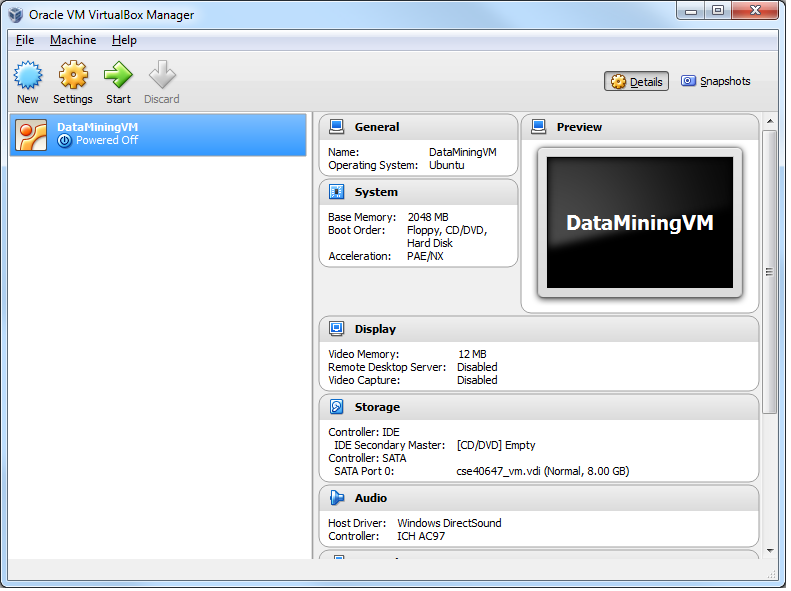
\includegraphics[scale=0.6]{img1.png}
	\caption{What you should see after successfully creating your VM from the provided VDI file.}
\end{figure}

\vspace{12pt}

When the process is complete, what you see should be roughly identical to the above window. Now select the DataMiningVM and click \textit{Start}. When the machine boots, you will log in using the \textbf{student} account. The password for that account is \textbf{student}.

\vspace{8pt}

Done! That's it. You have everything you need.

\vspace{8pt}
\subsection*{Step 3 \textemdash~Submission}

Create an IPython Notebook and run the code in Listing 1 with any modifications you desire (e.g., print your name somewhere). Be sure to modify/add at least one line.

\vspace{8pt}

To create a new IPython Notebook, you simply need to open the terminal and run the following command:

\begin{center}
\texttt{ipython notebook \--\--pylab inline}
\end{center}

This will bring up the IPython web interface from where you may select \textit{New Notebook}. Once you are finished, rename your Notebook \textbf{yourNetID\_assignment0} and save it by going to \mbox{File $\rightarrow$ Download as $\rightarrow$ IPython}. This will generate an .ipynb file. Place this file in your dropbox at:

\begin{center}
\texttt{/afs/nd.edu/courses/cse/cse40647.01/dropbox/yourNetID}
\end{center}

The final notebook should be similar to this one \href{http://nbviewer.ipython.org/github/cse40647/cse40647/blob/sp.14/assignment0/assignment0_sol.ipynb}{here}.

\clearpage
\section{Using your personal machine}

Ensure that your machine has the following software installed:

\begin{itemize}
\item Python 2.7.3
\item NumPy 1.8.0
\item SciPy (library) 0.9.0
\item Matplotlib 1.3.1
\item pandas 0.12.0
\item IPython 1.1.0
\item scikit-learn 0.14.1
\end{itemize}

Complete this assignment by following \textit{Step 3} above.

\clearpage

\perlscript{code}{Sample Python code for testing required modules}

\end{document} 